\chapter{Fundamentals}
\section{Virtualisation}
\subsection{Axioms}
\label{ch:fundamentals/virtualisation/axioms}
\subsubsection{Noninterference}
\label{ch:fundamentals/virtualisation/axioms/noninterference}
\textcite{10.1145/368481.368502} summarise the fundamental requirements of a multiprogramming 
system and emphasise the concept of noninterference between processes across space and time. 
\textit{Spatial noninterference} is represented by all mechanisms that protect references to memory, 
disk and input-output devices \cite{10.1145/368481.368502}. For example, memory segmentation 
is a method found in operating system kernels that assigns each process a dedicated portion
of physical memory that is invisible to all other processes in the system. The kernel traps 
any attempt made by a process to access memory outside its allocated memory segment, thereby 
guaranteeing spatial noninterference \cite{10.5555/2490781}. \textit{Temporal noninterference} refers
to those mechanisms that allocate execution time and protect against the monopolisation thereof 
\cite{10.1145/368481.368502}. For instance, CPU scheduling is a technique that decides which process 
shall run on a core such that the core does not idle and all processes make sufficient 
runtime progress \cite{10.5555/2490781}. The scheduling semantics, paired with an interrupt mechanism 
that makes sure that no process has hold of the core for too long, guarantee temporal noninterference.

\subsubsection{Isolation}
\label{ch:fundamentals/virtualisation/axioms/isolation}
\textcite{10.1145/3381052.3381315} define isolation as the level of dependency that a virtualisation 
platform has towards the host kernel. We generalise this definition and say that \textit{isolation} 
is the level of dependency that one piece of software has to another. Conceptually, isolation 
deals with explicit vertical relationships between software, and noninterference deals with 
implicit horizontal relationships between processes. The level of dependency can be quantified by 
counting the lines of external code that a software executes to obtain the desired functionality. 
For example, \textcite{10.1145/3381052.3381315} count the lines of kernel code 
that a virtualisation platform executes when providing services to sandboxed applications. 
High counts indicate a strong dependency, i.e weak isolation.  

\subsubsection{Performance}
\label{ch:fundamentals/virtualisation/axioms/performance}
\textcite{10.1145/3365199} defines performance as the contention between the overhead associated 
with isolating a process from its environment and the benefits of sharing resources between processes,
i.e fully utilising the capacity of the underlying resource pool. \textcite{10.1145/3381052.3381315}
use a similar definition and measure the level of isolation provided by three different virtualisation 
platforms contrasted against processing unit, memory and input-output performance metrics. 
Isolation is measured as described in Chapter \ref{ch:fundamentals/virtualisation/axioms/isolation}.
The lines of code are mapped to the kernel 
subsystem in which they reside, resulting in an isolation metric per subsystem.
Workloads are then executed as sandboxed applications, instantiated multiple times to measure resource 
utilisation on a single host system, and compared against the lines of code executed by the subsystem 
that the workload corresponds to. For example, the authors define an application that computes prime numbers up 
to a limit. Since the workload is compute-bound, processing speed is measured and compared to the 
number of lines of executed code that reside in the processing unit and architecture-specific subsystems of
the kernel.

\textcite{10.1145/3132747.3132763} use \textit{same-host density} as a performance metric that measures 
the number of sandboxed applications that can be consolidated onto a single server.
The authors \enquote{sequentially start 1000 virtual machines and measure the time it takes to
create each VM and the time it takes the VM to boot} \cite[5]{10.1145/3132747.3132763}. 
Virtual machines are described in Chapter \ref{ch:fundamentals/virtualisation/hardware-virtualisation}.
In addition, \textit{boot, pause and unpause times} are also considered as important performance indicators for particular 
use cases, such as elastic content delivery networks \cite{10.1145/3050748.3050757} \cite{10.1145/3132747.3132763}.

\subsection{Hardware Virtualisation}
\label{ch:fundamentals/virtualisation/hardware-virtualisation}
\textcite{10.1145/361011.361073} refer to the control program as a \textit{virtual machine monitor} that 
ensures isolation and noninterference by providing every program with an environment that is \enquote{[...] effect
identical with that demonstrated if the program had been run on the original machine directly} 
\cite[2]{10.1145/361011.361073}. This definition implies that a running program does not directly use
the bare metal resources available. Instead, resources are emulated by the virtual machine monitor at
the instruction level and presented as a dedicated physical system. Such an environment is called 
a \textit{virtual machine}.

\textcite{10.1145/361011.361073} define a requirement that the instruction-set architecture of a computer
has to satisfy for it to be virtualisable. The instruction set must be segregated into three groups of
instructions - privileged, sensitive and innocuous. An instruction is privileged if it requires changing
the mode of execution from user to supervisor mode by means of a trap \cite{10.1145/361011.361073}. 
An instruction $i$ is control-sensitive if, when applied to the current processor state $S_1$, results
in a new state $i(S_{1}) = S_{2}$ such that the execution mode of $S_{2}$ does not equal that of $S_{1}$
or if $S_{2}$ has access to different resources than $S_1$ or both \cite{10.1145/361011.361073}. 
An instruction is behaviour-sensitive if its execution depends on the execution mode or its position
in memory \cite{10.1145/361011.361073}. An instruction is innocuous if it is not sensitive. 
Given these definitions, a computer is virtualisable \enquote{[...] if the set of sensitive instructions
for that computer is a subset of the set of privileged instructions} \cite[6]{10.1145/361011.361073}.
If this criterion is met, the virtual machine monitor can trap all sensitive instructions and emulate 
each via a homomorphism $i: C_{r} \rightarrow C_{v}$ that maps the state space of the processor without
the virtual machine monitor loaded $C_{r}$ to the state space with the virtual machine monitor loaded 
$C_{v}$ \cite{10.1145/361011.361073}. Innocuous instructions do not require protection, i.e a homomorphic
mapping, and are directly executed by the processor \cite{10.1145/361011.361073}.

The aforementioned homomorphism enables a virtual machine to host a kernel, referred to as a \textit{guest kernel}, that 
\enquote{believes} it is interacting with a physical system.
Consequently, the isolation and noninterference boundaries between user programs 
running on different virtual machines are stronger compared to user processes running on a shared kernel. 
Even if a guest kernel becomes compromised or encounters an unrecoverable error condition, 
other virtual machines remain unaffected.

The performance cost of hardware virtualisation becomes aparent when measuring same-host density. 
\subsection{Operating System Virtualisation}
\label{ch:fundamentals/virtualisation/os-virtualisation}

%\begin{figure}
%\centering
%    \begin{subfigure}[b]{0.45\textwidth}
%        \centering
%        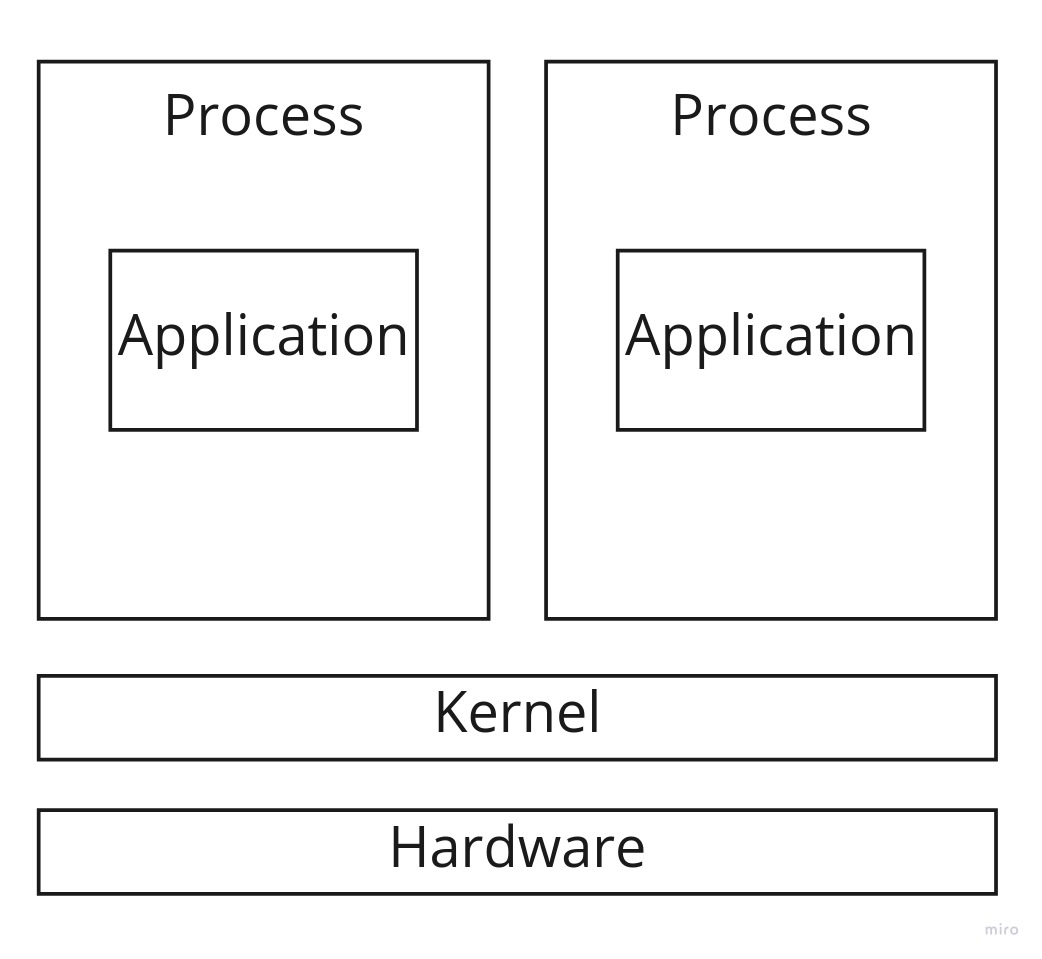
\includegraphics[width=0.6\textwidth]{images/fundamentals/kernel-virt-arch.jpg}
%        \caption{Virtualisation using a shared kernel that constantly assures noninterference by 
%                handling service requests from user processes. Kernel has full control of the system
%                and represents a single point of failure. There are no mechanisms to reestablsh 
%                system health.}
%        \label{images:fundamentals/kernel-virt-arch.jpg}
%    \end{subfigure}%
%    \hfill
%    \begin{subfigure}[b]{0.45\textwidth}
%        \centering
%        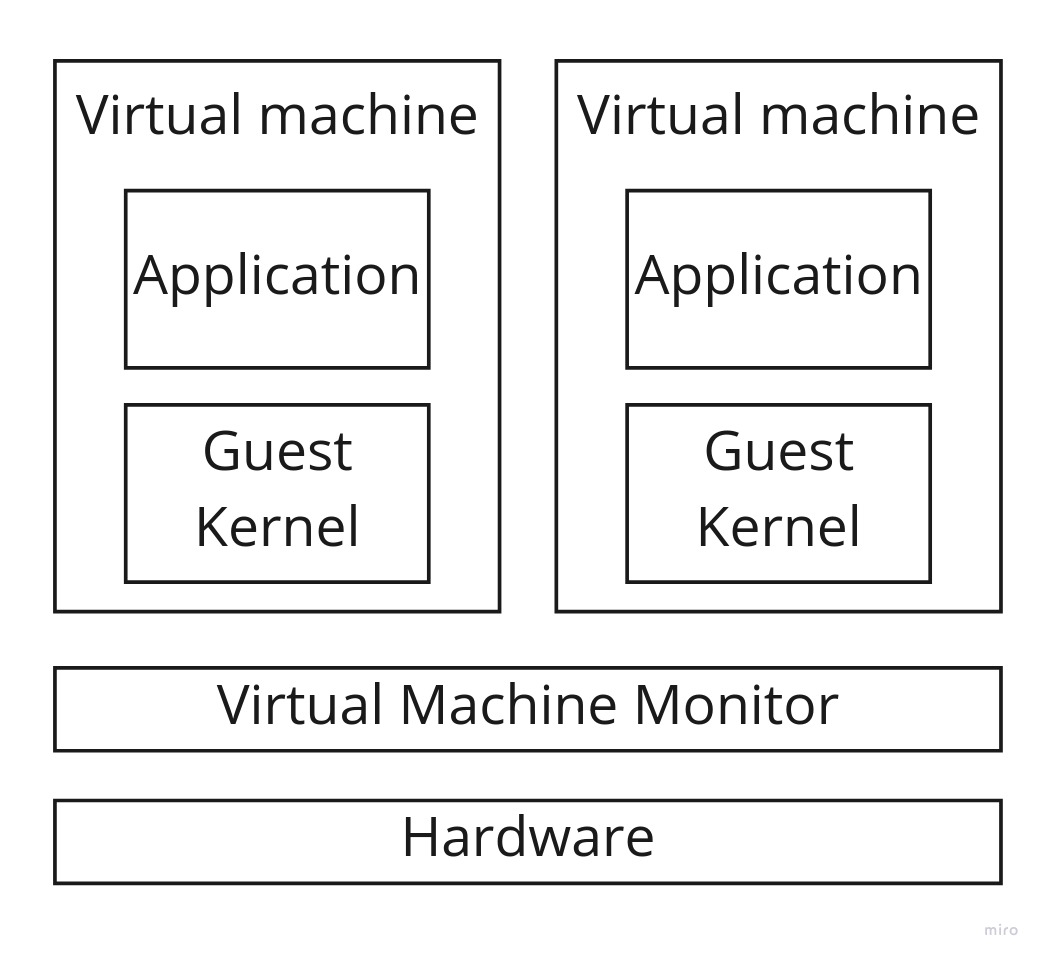
\includegraphics[width=0.6\textwidth]{images/fundamentals/full-virt-arch.jpg}
%        \caption{Virtualisation using multiple independent kernels, each ensuring noninterference. 
%                If one kernel fails, the virtual machine monitor can reclaim the respective resources or 
%                perform operations that reconstruct the virtual machine's state from a health checkpoint.}
%        \label{images:fundamentals/full-virt-arch.jpg}
%    \end{subfigure}
%\caption{Architectural comparison between shared-kernel virtualisation (\ref{images:fundamentals/kernel-virt-arch.jpg})
%         and multi-kernel virtualisation using a virtual machine monitor (\ref{images:fundamentals/full-virt-arch.jpg})}
%\label{images:fundamentals/virt-arch}
%\end{figure}

%The STRETCH system \cite{10.1145/368481.368502}, albeit quite old, employs an architecture used by 
%modern kernels to guarantee noninterference. The author describes an interruption system that can 
%transfer execution to a different memory address whenever a condition of the machine or process 
%changes, e.g an I/O device emits a signal or the process attempts divison by zero, respectively.
%The address holds the start instruction of a privileged routine that can react to the changed 
%condition. For example, the routine could serialise access to an I/O device, decode the bit stream 
%and copy it into a memory block local to the process that issued the request. Serialising access 
%ensures that concurrently executing processes cannot spatially interfere with the request. Scheduling
%the next request to be processed so that all programs make equal or similar runtime progress guarantees 
%temporal noninterference. It is important to note that, by definition, the kernel is considered 
%trustworthy and is allowed to access and modify space assigned to user processes. In other words, 
%noninterference between the kernel and user processes is not assured. Therefore, if the kernel is
%compromised or encounters an unrecoverable error condition, all user processes become untrustworthy 
%or unavailable, respectively.
